\section{Missing Details from the Experiments}\label{app_experiments}


\subsection{Synthetic Settings}\label{app_synthetic}
	We describe the parameters used for producing Figure \ref{fig_model_shift_phasetrans}.
	For all three simulations, we use dimension $p = 200$.
	In Figure \ref{fig_model_shift}, we use $\rho_1 = 90, \rho_2 = 30$ for sample sizes.
	The noise level is $\sigma = 5$.
	We set $\kappa = 1$ and vary model distance $d$ from $0.01$ to $0.2$.
	The $x$-axis measure the function $\Phi(\beta_1, \beta_2)$ described in Section \ref{sec_similarity}.
	In Figure \ref{fig_size}, we set $\kappa = 1$ and $d = 0.02$ for model distance.
	We use $\rho_2 = 500$ and vary $\rho_1$ from $50$ to $800$ for sample sizes.
	In Figure \ref{fig_covariate}, we set $\kappa = 1$ and $d = 0$.
	We set $\rho_2 = 4$ and vary $\rho_1$ from $5$ to $25$ for sample sizes.
	We use the scale parameter $\lambda = 1$ for the curve without covariate shift and $\lambda = 2$ for the curve with covariate shift (cf. Section \ref{sec_covshift}).
	Without loss of generality, we have rescaled the $x$ and $y$ axis for the ease of presentation.
	This can be achieved similarly by rescaling the task data.

\subsection{Image and Text Classification Settings}\label{app_it}

For the text classification experiment, we encode each word using the GLoVe word vectors.
\footnote{http://nlp.stanford.edu/data/wordvecs/glove.6B.zip}
We apply an average pooling layer over the word embeddings.
Then we add a multi-layer perception (MLP), LSTM, or CNN layer on top of the word embeddings \cite{lei2018simple}.

\textbf{Single-task based metric.}
We simplify the setup of this experiment by fixing the sample sizes of every task pair.
For sentiment analysis tasks, the source task uses xx training samples and the target task uses $1000$ training samples for every task pair.
For image classification tasks, the training sample size is 10,000 for every task.

\textbf{Incremental training schedule.}
For the case of two tasks, we compare the incremental training scheduled described in Algorithm \ref{alg_inc_train} below to a round-robin training schedule baseline.
We set the parameters of Algorithm \ref{alg_inc_train} using batch size $32$ and epochs $T = xx$.
The threshold $\tau$ is set as the accuracy of the target task using the baseline training schedule.

For the case of six tasks,

\begin{algorithm}[!h]
	\caption{An incremental training schedule for efficient multi-task learning with two tasks}
	\label{alg_inc_train}
	\begin{algorithmic}[1]
		\Input Two tasks $(X_1, Y_1)$ and $(X_2, Y_2)$.
		\Param A shared module $B$, output layers $W_1, W_2$ as in the hard parameter sharing architecture.
		\Req \# batches $S$, epochs $T$, task $2$'s validation accuracy $\hat{g}(B; W_2)$, a threshold $\tau\in(0,1)$.
		\Output The trained modules $B, W_2$ optimized for task $2$.
		\State Divide $(X_1, Y_1)$ randomly into $S$ batches: $(x^{(1)}, y^{(1)}), \dots, (x^{(S)}, y^{(S)})$.
		\For{$i = 1,\dots, S$}
			\For{$j = 1,\dots, T$}
				\State Update $B, W_1, W_2$ using the training data $\set{x^{(k)}, x^{(k)}}_{k=1}^i$ and  $(X_2, Y_2)$.
			\EndFor
			\State Let $a_i = \hat{g}(B; W_2)$ be the validation accuracy.
			\If{$a_i < a_{i-1}$ or $a_i > \tau$}
				\State \textbf{break}
			\EndIf
		\EndFor
	\end{algorithmic}
\end{algorithm}




\textbf{Theoretical validation.}
For Figure \ref{fig_ab_sim}, \todo{how do we select each task pair?}
For Figure \ref{fig_ab_data} and Figure \ref{fig_ab_cov}, the sample size of the target task is fixed as $1000$.
We vary the sample size of the source task from $100$ to $3000$.


%We validate that MTL performs better when the source task is more similar to the target task.
%We show the result on the sentiment analysis tasks.
%For a target task, we manually select a similar task and a dissimilar task based on prior knowledge.
%Figure \ref{fig_ab_sim} confirms the result.
%Recall that Section \ref{sec_data_size} shows that increasing the data size of the source task does not always improve the performance of MTL for the target task.
%In Figure \ref{fig_ab_data}, we show that for source task MR and target task SST, there is a transition from positive to negative transfer as we increase the data size of the source task.
%Our result provides a fine-grained insight on the covariance alignment algorithm proposed in \cite{WZR20}.
%Recall that the covariance alignment procedure in \cite{WZR20} adds an additional module between the word embedding representation and the shared module.
%When the source task data size is particularly large compared to the target task, we show that applying the covariance alignment algorithm results in more significant gains.
%In Figure \ref{fig_ab_cov}, we observe that the benefit from aligning task covariances becomes more significant for LSTM and MLP as we increase the number of datapoints of the source task.

\iffalse
\textbf{Further results on covariance alignment.}
%Note: For text classification tasks, the source task training data size ranges from 500 to 1,500 and target task training data size is 1000; For ChestX-ray14,

\begin{figure}[!h]
	\centering
	\begin{subfigure}[b]{0.48\textwidth}
		\centering
		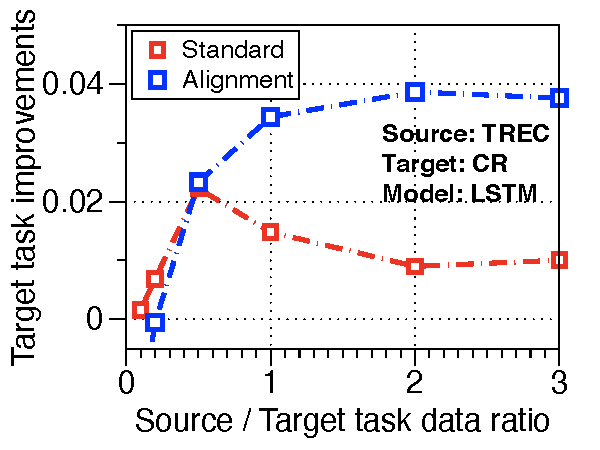
\includegraphics[width=0.75\textwidth]{figures/ratio_alignment_norm_trec_cr_lstm.pdf}
		\caption{Task pair TREC and CR}
	\end{subfigure}\hfill
		\begin{subfigure}[b]{0.48\textwidth}
		\centering
		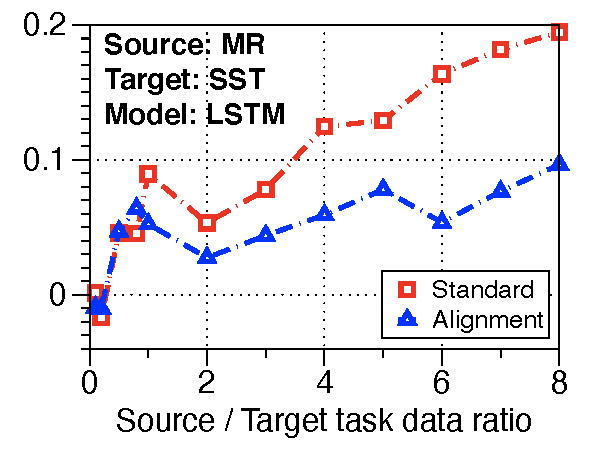
\includegraphics[width=0.75\textwidth]{figures/ratio_alignment_mr_sst_lstm.pdf}
		\caption{Task pair MR and SST}
	\end{subfigure}
	\caption{(a) For the task pair TREC and CR, adding the covariance alignment procedure provides more improvement when the source/target sample ratio is large.
	(b) For the task pair MR and SST, adding the covariance alignment procedure hurts performance. We suspect that this happens because of overfitting on the extra parameters in the additional covariance alignment module.}
	\label{fig_covariate_app}
\end{figure}
\fi
